% in Terminal enter
% Rscript -e "library(knitr); knit('presentation.Rnw')"
% pdflatex presentation
% biber presentation
% pdflatex presentation
% pdflatex presentation
% 
% Einleitung
% 
% Überblick children kurz
% Wie fördern sie
% Über d verteilt
% Beide programme erklären
% Daten sammlung prozess
% Datenstruktur
% Datenaufbereitung
% 
% Summary Statistics
% 
% Mittagstisch
% Entdeckerfonds
% Subsidy
% Selfworth
% Daytodayskills
% Health variables
% 
% Regressionen
% 
% DiD-Ansatz
% 
% Grundlegende Idee – was wollen wir testen?
% Zielvariablen und warum
% Grafische evidenz 
% Resultate - Regressionstabellen
% 
% Fazit und Verbesserungsvorschläge
% 
% Gründe für fehlende effekte 
% Tipps zur datenerhebung und struktur
% partition


% when you begin a slide with a table or figure on it, always write
% \begin{frame}[fragile]
% the fragile option is important

% to make tables and figures fit, use
% scalebox = '0.75'
% or another number

% https://github.com/yihui/knitr/blob/master/inst/examples/knitr-beamer.Rnw



\documentclass{beamer}\usepackage[]{graphicx}\usepackage[]{color}
% maxwidth is the original width if it is less than linewidth
% otherwise use linewidth (to make sure the graphics do not exceed the margin)
\makeatletter
\def\maxwidth{ %
  \ifdim\Gin@nat@width>\linewidth
    \linewidth
  \else
    \Gin@nat@width
  \fi
}
\makeatother

\definecolor{fgcolor}{rgb}{0.345, 0.345, 0.345}
\newcommand{\hlnum}[1]{\textcolor[rgb]{0.686,0.059,0.569}{#1}}%
\newcommand{\hlstr}[1]{\textcolor[rgb]{0.192,0.494,0.8}{#1}}%
\newcommand{\hlcom}[1]{\textcolor[rgb]{0.678,0.584,0.686}{\textit{#1}}}%
\newcommand{\hlopt}[1]{\textcolor[rgb]{0,0,0}{#1}}%
\newcommand{\hlstd}[1]{\textcolor[rgb]{0.345,0.345,0.345}{#1}}%
\newcommand{\hlkwa}[1]{\textcolor[rgb]{0.161,0.373,0.58}{\textbf{#1}}}%
\newcommand{\hlkwb}[1]{\textcolor[rgb]{0.69,0.353,0.396}{#1}}%
\newcommand{\hlkwc}[1]{\textcolor[rgb]{0.333,0.667,0.333}{#1}}%
\newcommand{\hlkwd}[1]{\textcolor[rgb]{0.737,0.353,0.396}{\textbf{#1}}}%
\let\hlipl\hlkwb

\usepackage{framed}
\makeatletter
\newenvironment{kframe}{%
 \def\at@end@of@kframe{}%
 \ifinner\ifhmode%
  \def\at@end@of@kframe{\end{minipage}}%
  \begin{minipage}{\columnwidth}%
 \fi\fi%
 \def\FrameCommand##1{\hskip\@totalleftmargin \hskip-\fboxsep
 \colorbox{shadecolor}{##1}\hskip-\fboxsep
     % There is no \\@totalrightmargin, so:
     \hskip-\linewidth \hskip-\@totalleftmargin \hskip\columnwidth}%
 \MakeFramed {\advance\hsize-\width
   \@totalleftmargin\z@ \linewidth\hsize
   \@setminipage}}%
 {\par\unskip\endMakeFramed%
 \at@end@of@kframe}
\makeatother

\definecolor{shadecolor}{rgb}{.97, .97, .97}
\definecolor{messagecolor}{rgb}{0, 0, 0}
\definecolor{warningcolor}{rgb}{1, 0, 1}
\definecolor{errorcolor}{rgb}{1, 0, 0}
\newenvironment{knitrout}{}{} % an empty environment to be redefined in TeX

\usepackage{alltt}
% \usepackage{lmodern}
% \usepackage{lscape}
% \usepackage{graphicx}
% \usepackage[utf8]{inputenc}
\usepackage[backend=biber, bibstyle=apa, citestyle=authoryear]{biblatex}
% \usepackage{floatrow}
% \usepackage{booktabs}
% \usepackage{rotating}
% \usepackage{dcolumn}
% \usepackage{mathtools}
% \usepackage[left = 2.5cm, top = 2.5cm, right = 2.5cm, bottom = 2.0cm]{geometry}
% \usepackage[hidelinks]{hyperref}
% \usepackage{mathtools}
% \usepackage{amssymb}
% \usepackage{latexsym}
% \usepackage{eurosym}
% \usepackage{xcolor}
% \usepackage{graphicx}
% \usepackage{dcolumn}
% \usepackage{floatrow}
% \usepackage[english]{babel}
% \usepackage[utf8]{inputenc}
% \usepackage{subfigure}
% \usepackage[flushleft]{threeparttable}
% \usepackage{booktabs}
% \usepackage{adjustbox}
% \usepackage{sidecap}
% \usepackage{ifthen}
% \usepackage[backend=biber, bibstyle=apa, citestyle=authoryear]{biblatex}
% \usepackage[hidelinks]{hyperref}
% \graphicspath{{./Visuals/}}
% \setcounter{secnumdepth}{3}
% \setcounter{tocdepth}{3}
% \usepackage{url}
% \ifx\hypersetup\undefined
%   \AtBeginDocument{%
%     \hypersetup{unicode=true,pdfusetitle,
%  bookmarks=true,bookmarksnumbered=false,bookmarksopen=false,
%  breaklinks=false,pdfborder={0 0 0},pdfborderstyle={},backref=false,colorlinks=false}
%   }
% \else
%   \hypersetup{unicode=true,pdfusetitle,
%  bookmarks=true,bookmarksnumbered=false,bookmarksopen=false,
%  breaklinks=false,pdfborder={0 0 0},pdfborderstyle={},backref=false,colorlinks=false}
% \fi
% \usepackage{breakurl}
% 
% \makeatletter
%
% Fancy fit image command with optional caption copied from https://www.patrickbaylis.com/posts/2018-10-11-beamer-resizing/
% \makeatletter
% \newcommand{\fitimage}[2][\@nil]{
% 	\begin{figure}
% 		\begin{adjustbox}{width=0.9\textwidth, totalheight=\textheight-2\baselineskip-2\baselineskip,keepaspectratio}
% 			\includegraphics{#2}
% 		\end{adjustbox}
% 		\def\tmp{#1}%
% 		\ifx\tmp\@nnil
% 		\else
% 		\caption{#1}
% 		\fi
% 	\end{figure}
% }
% \makeatother
% 
% \rmfamily

\usetheme{CambridgeUS}

\usecolortheme{crane}

\addbibresource{references.bib}

%
\IfFileExists{upquote.sty}{\usepackage{upquote}}{}
\begin{document}




\title[Analyse der Survey-Daten von CHILDREN]{Analyse der Survey-Daten von CHILDREN for a better World e.V.
	}
\author[Laura, Laura, Jonathan, Rafael und Yannick]{
Laura Huber\\
\and
Laura Jepsen\\
\and
Jonathan Kirschner\\
\and
Rafael Schütz\\
\and
Yannick Zurl\\
\and
Studentisches Praxisprojekt zur Empirischen Wirtschaftsforschung PaRE3To\\
\and
Ludwig-Maximilians-Universität München}
\date{3. März 2020}


\begin{frame}
	\maketitle
\end{frame}

\frame{\frametitle{Table of Contents}
	\tableofcontents
}

\frame{\frametitle{List of Tables}
	\listoftables
}

\frame{\frametitle{List of Figures}
	\listoffigures
}

\section{Summary Statistics}

\begin{frame}[fragile]
\frametitle{Summary Statistics}
<<<<<<< HEAD
% latex table generated in R 3.5.1 by xtable 1.8-4 package
% Sun Mar 01 15:48:20 2020
=======
% latex table generated in R 3.6.2 by xtable 1.8-4 package
<<<<<<< HEAD
% Sun Mar  1 16:08:10 2020
=======
% Sun Mar 01 16:01:01 2020
>>>>>>> 04c95a6a74f6edfb10dafc0811e82cdd3d3a9024
>>>>>>> 7ccd638bd2873d0916b703596f58f6d1096d9d92
\begin{table}[ht]
\centering
\scalebox{0.75}{
\begin{tabular}{lccccc}
  \hline
 & Year & Beneficiaries, Meals & Beneficiaries, Trips & Organizations, Meals & Organizations, Trips \\ 
  \hline
1 & 2011 & 3748.0 &  & 52 &  \\ 
  2 & 2012 & 3556.0 & 2803.0 & 51 & 44 \\ 
  3 & 2013 & 4015.0 & 2823.0 & 55 & 42 \\ 
  4 & 2014 & 4685.0 & 2752.0 & 55 & 43 \\ 
  5 & 2015 & 5857.0 & 3823.0 & 55 & 49 \\ 
  6 & 2016 & 3075.0 & 3819.0 & 59 & 48 \\ 
  7 & 2017 & 4895.0 & 4150.0 & 64 & 48 \\ 
  8 & 2018 & 5102.5 & 6911.0 & 68 & 49 \\ 
   \hline
\end{tabular}
}
\caption{Summary Statistics} 
\label{fundamentalDynamics}
\end{table}


\end{frame}

<<<<<<< HEAD
\section{DID - Estimation}
=======
\begin{frame}[fragile]
\frametitle{Dynamics}

\begin{figure}
  \caption{Yearly dynamics of total grants in Meals and Trips program}
  \label{totalGrantsDyn}

\begin{knitrout}\footnotesize
\definecolor{shadecolor}{rgb}{0.969, 0.969, 0.969}\color{fgcolor}

{\centering 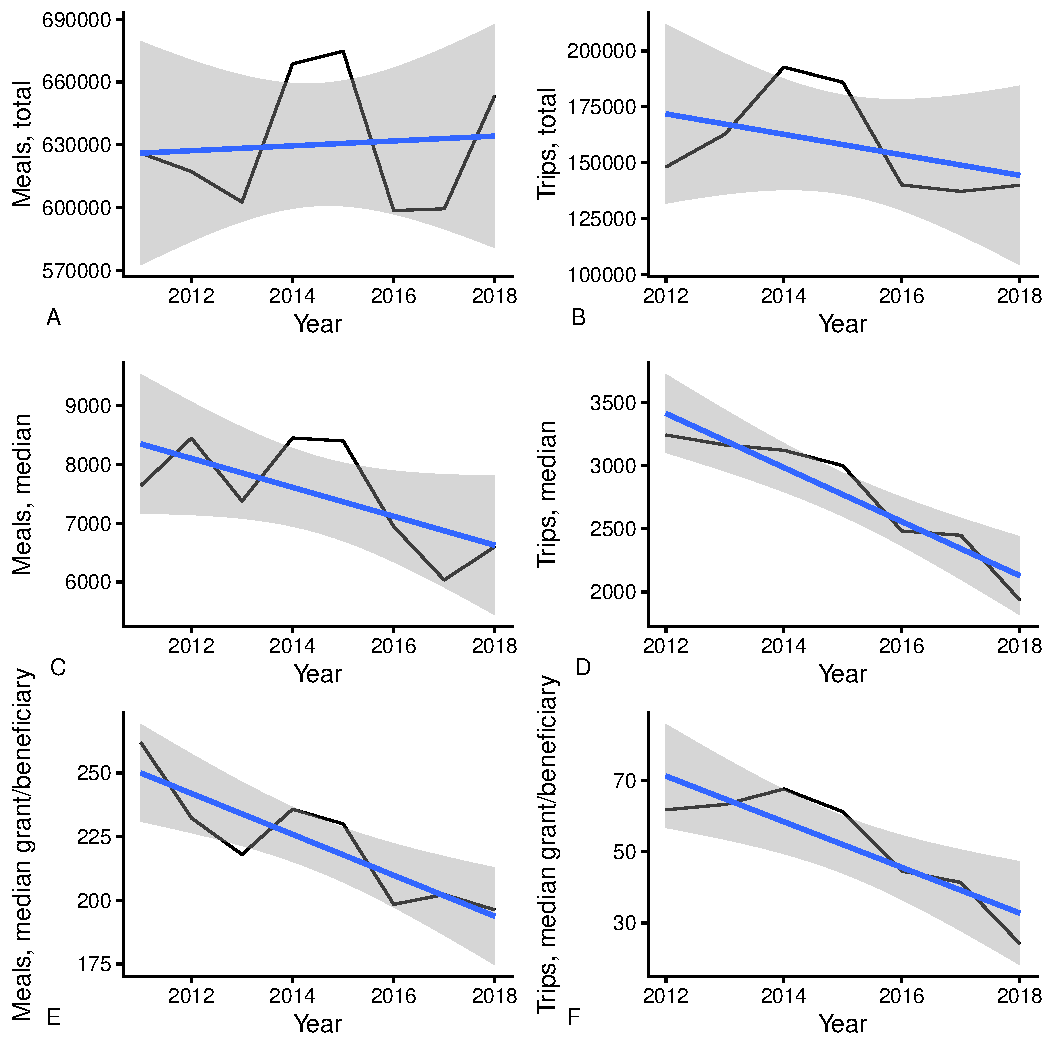
\includegraphics[width=\maxwidth]{figure/beamer-GrantTrend-1} 

}
>>>>>>> 7ccd638bd2873d0916b703596f58f6d1096d9d92

\begin{frame}[fragile]
\frametitle{Graphical evidence}
\end{frame}

\end{knitrout}

% \floatfoot{This graph shows the development of grants in the Meals compared to the Trips program. We distinguish between the sum of grants in one year, the median grant and the median grant per beneficiary. From left to right: Meals, Trips. From top to bottom: sum, median, median per beneficiary. We have deflated the values to 2015 euros using the price index related to food and non-alcoholic beverages(in German: Nahrungsmittel und alkoholfreie Getränke) for the Meals program and the price index related to Leisure, Entertainment and Culture (in German: Freizeit, Unterhaltung, Kultur) provided by the Federal Statistical Office of Germany (Statistisches Bundesamt).}
\end{figure}

\end{frame}


\frame[allowframebreaks]{\frametitle{References}
		\tiny
		\printbibliography
}
	
\end{document}


